ope\chapter{Tail-Anchored Protein Datasets}
\sloppy
% gls refers to a glossary term, cite refers to an entry from the separate bibtex folder. url is a lazy way of forcing monospaced text. textit is italics. sections and subsections are the headers.
\section{Abstract}

\section{Introduction}

~\gls{ta} proteins are a topologically distinct class of intracellular proteins defined by their single carboxy-terminal~\gls{tms} with a cytosolic facing amino-terminus.
~\gls{ta} proteins are involved in a range of key cellular functions including protein translocation and apoptosis.
Additionally, within the~\gls{ta} class of proteins are a set of vesicle fusion proteins called~\gls{snare} proteins.
There is biomedical interest in~\gls{snare} drug delivery mechanisms.
~\gls{snare}s can fuse liposomes containing various drug payloads into the membrane.

The pipeline generates a list of singlepass proteins with a transmembrane domain close to the C terminal, that are not splice isoforms.
A previous study by Kalbfleisch \textit{et al.} published in Traffic 2007 (8: 1687-1694) predicted 411 tail anchor proteins~\cite{Kalbfleisch2007}.
The tools developed herein are openly available for re-application to other datasets.
Notably, known~\gls{snare} transmembrane helices are highly hydrophobic even compared to other~\gls{ta} transmembrane helices.
We compare Kyte and Doolittle hydrophobicity profiles of our filtered human protein list against the profiles of previously known~\gls{snare} and~\gls{ta} proteins.
This provided a list of potential~\gls{snare} proteins in addition to potential spontaneously inserting~\gls{ta} proteins similar to cytochrome b5 which have the least hydrophobic transmembrane helices.

Tail-anchored proteins are a topologically distinct class of intracellular proteins defined by their single carboxy-terminal transmembrane domain with a cytosolic-facing amino-terminus.
%Need a figure here of a crystal structure TA.

Tail-anchored proteins are involved in a range of key cellular functions including protein translocation and apoptosis.
Additionally, within the tail-anchored class of proteins are a set of vesicle fusion proteins called \gls{snare} proteins.
There is biomedical interest in \gls{snare} drug delivery mechanisms.

\gls{snare}s can fuse liposomes containing various drug payloads into the membrane.
Notably, known \gls{snare} \gls{tmh}s are highly hydrophobic even compared to other tail anchored \gls{tmh}s~\cite{Kalbfleisch2007}.
This hydrophobicity appears to be a determinate factor in the precise delivery mechanistic route that a~\gls{ta} proteins use for insertion~\cite{Rabu2008, Rabu2009}, for which there is evidence demonstrating that are several mechanisms~\cite{Rabu2009, Johnson2013}.

Whilst most eukaryotic~\gls{ta} proteins are inserted into the~\gls{er}.

\section{Results}

\subsection{Tail-Anchored Protein Datasets Are A Moving Target}
Here, we use two sources for \gls{ta} protein datasets.
One dataset is based on a previous method~\cite{Kalbfleisch2007} to obtain \gls{ta} datasets and consists of 9296 \gls{tmh} residues (13279 including up to $\pm$5 flanking residues) from 443 SwissProt entries with 90\% redundancy removal.
Another dataset contains the UniProt curated set of Type IV membrane proteins again with 90\% redundancy removal.
This dataset contains 21119 \gls{tmh} residues (28791 including uptt to $\pm$5 flanking residues) from 987 UniProt protein records.

We compared redundant versions of these two datasets to the S1 dataset from a previous method~\cite{Kalbfleisch2007}, that aimed to gather \gls{ta} proteins in the human genome from the NCBI, to see how many records are shared, how many are now obselete, and how many are unique.

% Venn diagram
\begin{figure}[!ht]
\centering
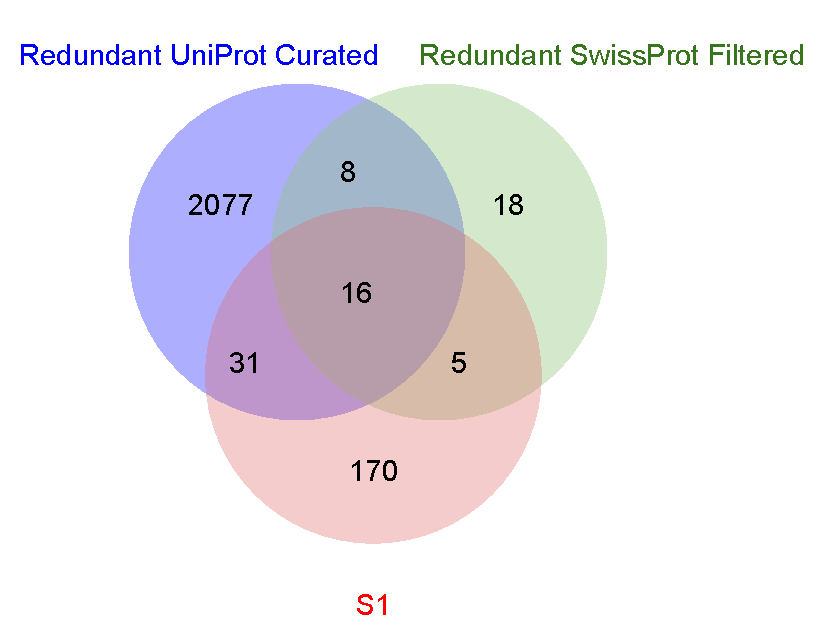
\includegraphics[width=0.5\textwidth]{TA_chapter/database-overlap}
		\captionof{figure}[A venn diagram showing tail anchored protein UniProt ids present in each of the datasets as well as those present in multiple datasets.]{\textbf{A venn diagram showing tail anchored protein UniProt ids present in each of the datasets as well as those present in multiple datasets.}
The number of ids present in redundant versions of
i) the supplementary materials table of a previous study predicting the complete set of human tail anchored proteins denote by S1~\cite{Kalbfleisch2007},
ii) the Swissprot dataset filtered according to typical~\gls{ta} features limited to the human proteome~\cite{TheUniProtConsortium2014}, and
iii) The UniProt curated list of~\gls{ta} proteins~\cite{TheUniProtConsortium2014}.
Note that to avoid losing IDs to redundancy reduction this diagram was generated without the use of CD-HIT~\cite{Huang2010, Wu2011}, which is applied in later statistical analysis.}

\label{fig:tadatasetoverlap}
\end{figure}

Figure~\ref{fig:tadatasetoverlap} shows that already a study from 2007~\cite{Kalbfleisch2007} has 175 record ids of 222 records (78.8\%) that do not share overlap the up-to-date manually curated UniProt dataset~\cite{TheUniProtConsortium2014}.
Of the 166 unique records of that 2007 dataset, 92 records do have location annotation in UniProt that the scripts herein use for topological determination, leaving 74 records without location annotation.
This leaves 92 of 222 (41.4\%) records that originally fitted criteria that no longer fit those same criteria.
If we exclude those lacking suitable annotation i.e ids from S1 that are found in either SwissProt with the filters (9), the curated UniProt list (14), or both (33), compared to the 92 that have annotation contradicting the original prodictions, 37.8\% of the ids overlap.

Equivalent criteria were applied to the entire SwissProt database and then restricted to the human proteome dataset.
43 of these 77 records (55.8\%) are in the curated UniProt~\gls{ta}  dataset leaving 34 records that meet the criteria out of the manually curated set (44.2\%of the filtered Swissprot dataset).
42 of the 77 (54.5\%) records from SwissProt filtered human dataset can be found in the original S1 list.
A further consideration is that, after removing redundant proteins, this method picked up  46 Archaeal and 66 bacterial records.

Datasets are a moving target as they are constantly updated with more accurate and reliable tools.
Perhaps unsurprisingly, as a trend, this shows that up-to-date datasets improve the reliability of this automated predicted method and that there is a large degree of what we now believe to be mistakes that occured in older prediction tools.
These automated criteria still do not fully align with the manually curated list, which is bound to change too, especially considering only 973 of a non-redundant (90\% CD-HIT threshold \cite{Huang2010, Wu2011}) set of those 2460 proteins of the UniProt manually curated set contained annotation for the transmembrane boundary residues.

Note that these numbers are not absolutely certain.
The greatest source of uncertainty here is that the original S1 list includes 411 records, however only 222 of these were successfully mapped to the UniProt dataset.
This figure is closer to the 202 proteins from the original list that excluded proteins that were either hypothetical or splice isoforms.
That being said, this ``conversion'' step prevents us from directly comparing the entire original S1 dataset.

\subsection{Species Variation}
% Average lines for figure, table for stats
\begin{figure}[!ht]
\centering
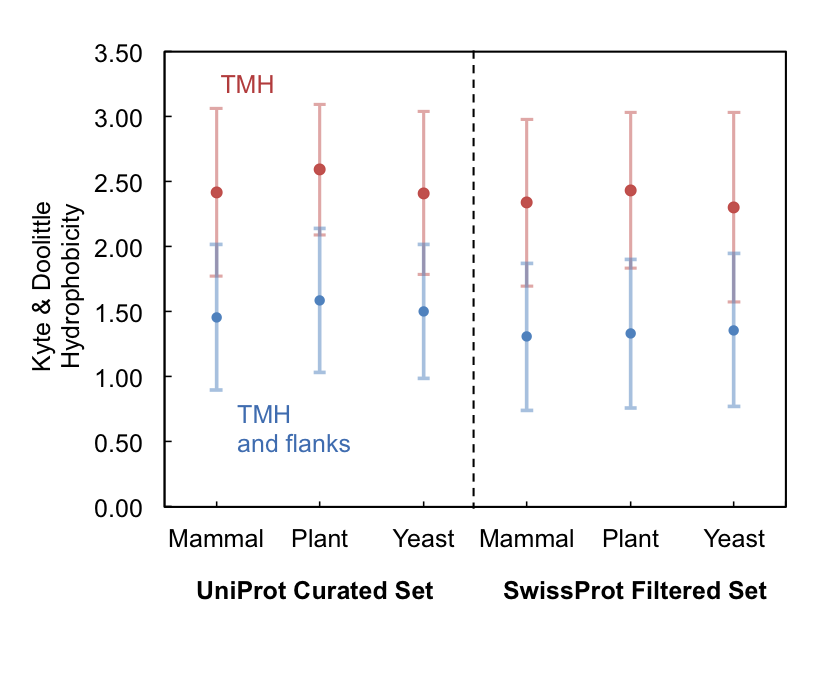
\includegraphics[width=1\textwidth]{TA_chapter/species-hydrophobicity}
\captionof{figure}[Average values of species datasets from UniProt manually curated set and SwissProt automatically filtered dataset.]
{\textbf{Average values of species datasets from UniProt manually curated set and SwissProt automatically filtered dataset.}

The average hydrophoicity values from the Kyte \& Doolittle scale ~\cite{Kyte1982} and the GlobProt scale \cite{Linding2003} for both the \gls{tmh} and the \gls{tmh}$\pm$5 residues. Values are shown for both the UniProt manually curated set and the SwissProt filtered set. In the UniProt manually curated set we compare the mammalian set of \gls{ta} proteins (Human N=38 and Mouse N=37) to \textit{A. thaliana} (N=60) representing plants  and  \textit{S. cerevisiae} (N=31) representing yeasts. For the SwissProt filtered set we compare the mammalian set of \gls{ta} proteins (Human N=46 and Mouse N=48) to \textit{A. thaliana} (N=49) representing plants  and  \textit{S. cerevisiae} (N=24) representing yeasts.
Error bars are shown at $\pm 1 \sigma$ from the mean of the respective dataset.
}

\label{fig:average_species_hydrophobicity_ta}
\end{figure}

When comparing the average Kyte \& Doolittle~\cite{Kyte1982} hydrophobicity values for the~\gls{tmh}s from humans and mice, \textit{A. thaliana}, and  \textit{S. cerevisiae}, we can see little difference between the mean values.
All of the mean values lie between $\sim$2.3-2.6 when we only consider the \gls{tmh} and at $\sim$1.3-1.6 when considering residues in close proximity to the~\gls{tmh} ($\pm$5 residues) (Figure~\ref{fig:average_species_hydrophobicity_ta}).
Indeed, we see no strong observable statistical differences in hydrophobicity ($P-value>8.30E-02$ in the UniProt curated list Table \ref{table:speciestableuniprotstats}, $P>3.35E-01$ in the SwissProt automatically filtered list Table \ref{table:speciestableswissprotstats}).

In single-pass proteins of Eukaryotic species there are typically various adaptations of the \gls{tmh} to adhere to the membrane constraints of the specific membrane that can be observed in terms of hydrophobicity~\cite{Sharpe2010}, especially in \gls{tmh} anchors~\cite{Baker2017}.
However, in these \gls{ta} protein datasets we see no such patterns at this sample size.

Here, we are dealing with datasets at least an order of magnitude smaller than those broad studies which could explain the absence of the effect.
However this only goes to show that if there is an effect in \gls{ta} proteins, it is indeed weak.

\begin{table}[htbp]
\centering
\captionof{table}[Hydrophobicity statistical comparisons between mouse and human, yeast, and plants in the SwissProt Filtered Dataset.]
{\textbf{Hydrophobicity statistical comparisons between mouse and human, yeast, and plants in the SwissProt Filtered Dataset.}
Here, we compare a mammalian set of \gls{ta} proteins (Human N=46 and Mouse N=48) to \textit{A. thaliana} (N=49) representing plants  and  \textit{S. cerevisiae} (N=24) representing yeasts.
The hydrophobicity was predicted as the mean average of the values of the sequences of the \gls{tmh}, as well another group including up to $\pm$5 flanking residues predicting the boundary of \gls{tmh}s is difficult, according to the Kyte \& Doolittle hydrophobicity scale~\cite{Kyte1982}.
%Disorder was calculated in the same way using the GlobProt scale \cite{Linding2003}.
The Test column refers to the statistical score obtaineed from the test; H statistic for the Kruskal Wallis, the KS statistic for the Kolmogorov Smirnov test, and the t-statistic for the T-test.
$P$ is the P-value of that statistical score.
$B$ refers to the Bahadur slope, an interpretation of the P-value that accounts for the sample size powering the test~\cite{Bahadur1967, Bahadur1971}.}
\tiny
	% Table generated by Excel2LaTeX from sheet 'SwissProt filtered species'

    \begin{tabular}{clrrrrrrrrr}
          &       & \multicolumn{3}{c}{Mammal and Plant} & \multicolumn{3}{c}{Mammal and Yeast} & \multicolumn{3}{c}{Plant and Yeast} \\
          &       & \multicolumn{1}{l}{ Test} & \multicolumn{1}{l}{ $P$} & \multicolumn{1}{l}{ $B$} & \multicolumn{1}{l}{ Test} & \multicolumn{1}{l}{ $P$} & \multicolumn{1}{l}{ $B$} & \multicolumn{1}{l}{ Test} & \multicolumn{1}{l}{ $P$} & \multicolumn{1}{l}{ $B$} \\
    \multirow{3}[0]{*}{TMH } &  Kruskal-Wallis & 0.93  & 3.35E-01 & 7.64E-03 & 0.10  & 7.56E-01 & 2.37E-03 & 0.84  & 3.60E-01 & 1.40E-02 \\
          &  Kolmogorov-Smirnov & 0.13  & 6.36E-01 & 3.17E-03 & 0.12  & 9.24E-01 & 6.69E-04 & 0.19  & 5.28E-01 & 8.76E-03 \\
          &  Student's T-test & -0.86 & 3.90E-01 & 6.58E-03 & 0.21  & 8.31E-01 & 1.57E-03 & 0.79  & 4.33E-01 & 1.15E-02 \\
    \multirow{3}[0]{*}{TMH and flanks } &  Kruskal-Wallis & 0.04  & 8.52E-01 & 1.12E-03 & 0.12  & 7.28E-01 & 2.69E-03 & 0.04  & 8.33E-01 & 2.51E-03 \\
          &  Kolmogorov-Smirnov & 0.11  & 7.72E-01 & 1.81E-03 & 0.13  & 8.79E-01 & 1.09E-03 & 0.11  & 9.80E-01 & 2.81E-04 \\
          &  Student's T-test & -0.22 & 8.23E-01 & 1.37E-03 & -0.38 & 7.04E-01 & 2.97E-03 & -0.19 & 8.50E-01 & 2.22E-03 \\
    \end{tabular}%
				\label{table:speciestableswissprotstats}

\end{table}%

\begin{table}[htbp]
\centering
\captionof{table}[Hydrophobicity statistical comparisons between mouse and human, yeast, and plants in the UniProt Curated Dataset.]
{\textbf{Hydrophobicity statistical comparisons between mouse and human, yeast, and plants in the UniProt Curated Dataset.}
Here, we compare a mammalian set of \gls{ta} proteins (Human N=38 and Mouse N=37) to \textit{A. thaliana} (N=60) representing plants  and  \textit{S. cerevisiae} (N=31) representing yeasts.
The hydrophobicity was predicted as the mean average of the values of the sequences of the \gls{tmh}, as well another group including up to $\pm$5 flanking residues predicting the boundary of \gls{tmh}s is difficult, according to the Kyte \& Doolittle hydrophobicity scale~\cite{Kyte1982}.
%Disorder was calculated in the same way using the GlobProt scale \cite{Linding2003}.
The Test column refers to the statistical score obtaineed from the test; H statistic for the Kruskal Wallis, the KS statistic for the Kolmogorov Smirnov test, and the t-statistic for the T-test.
$P$ is the P-value of that statistical score.
$B$ refers to the Bahadur slope, an interpretation of the P-value that accounts for the sample size powering the test~\cite{Bahadur1967, Bahadur1971}.}
	\tiny
	% Table generated by Excel2LaTeX from sheet 'SwissProt filtered species'

    \begin{tabular}{clrrrrrrrrr}
	          &       & \multicolumn{3}{c}{Mammal and Plant} & \multicolumn{3}{c}{Mammal and Yeast} & \multicolumn{3}{c}{Plant and Yeast} \\
	          &       & \multicolumn{1}{l}{ Test} & \multicolumn{1}{l}{ $P$} & \multicolumn{1}{l}{ $B$} & \multicolumn{1}{l}{ Test} & \multicolumn{1}{l}{ $P$} & \multicolumn{1}{l}{ $B$} & \multicolumn{1}{l}{ Test} & \multicolumn{1}{l}{ $P$} & \multicolumn{1}{l}{ $B$} \\
	    \multirow{3}[0]{*}{TMH } &  Kruskal-Wallis & 2.15  & 1.42E-01 & 1.45E-02 & 0.22  & 6.39E-01 & 4.22E-03 & 2.30  & 1.30E-01 & 2.25E-02 \\
	          &  Kolmogorov-Smirnov & 0.17  & 2.86E-01 & 9.27E-03 & 0.15  & 6.32E-01 & 4.34E-03 & 0.24  & 1.69E-01 & 1.95E-02 \\
	          &  Student's T-test & -1.71 & 8.96E-02 & 1.79E-02 & 0.04  & 9.70E-01 & 2.86E-04 & 1.47  & 1.46E-01 & 2.11E-02 \\
	    \multirow{3}[0]{*}{TMH and flanks } &  Kruskal-Wallis & 2.17  & 1.41E-01 & 1.45E-02 & 0.14  & 7.13E-01 & 3.19E-03 & 0.59  & 4.41E-01 & 9.00E-03 \\
	          &  Kolmogorov-Smirnov & 0.21  & 8.30E-02 & 1.84E-02 & 0.10  & 9.62E-01 & 3.62E-04 & 0.14  & 8.00E-01 & 2.45E-03 \\
	          &  Student's T-test & -1.33 & 1.86E-01 & 1.25E-02 & -0.39 & 7.00E-01 & 3.36E-03 & 0.69  & 4.90E-01 & 7.83E-03 \\
	    \end{tabular}%
					\label{table:speciestableuniprotstats}
	\end{table}%


\subsection{Organelle Membrane Variation}
% Average lines for figure, table for stats

When we consider the \gls{ta} proteins at certain locations within the cell ignoring species, we see clear differences in the biochemistry of the \gls{tmh}.
In the UniProt manually curated dataset, the Kyte \& Doolittle hydrophobicity scores rage from 1.7 in mitochondria to 2.7 in the \gls{pm} (Figure \ref{fig:average_organelle_factors_ta}A).
Similarly, in the SwissProt filtered dataset the mitochondria lies at 1.9, but it appears to be the golgi apparatus that is the peak at 2.4.

With such a strong hydrophobic difference that, as we saw in the species, may not be solely accounted for by adaptation to the different membrane compositions, it is important to consider if a cryptic targetting signal exists within the \gls{tmh} themselves for \gls{ta} proteins.
The linguistic sequence entropy of the \gls{tmh} string as well as the disorder were also examined.
In terms of sequence entropy, there is a marked lack of entropy in the \gls{pm} subset (mean entropy = 3.12 in the \gls{tmh}, 2.6 including $\pm$5 flanking residues) from the UniProt curated dataset compared to the other organelle datasets (entropy $>$ 3.3 and $>$ 2.8 including the flanks).
However this stark difference cannot be observed in the SwissProt set.
This is unsurprising given that the hydrophobic nature of the \gls{tmh}s demands that certain residues must be overrepresented, which lowers the sequence entropy.
In this case, we have a highly hydrophobic set, the \gls{pm} UniProt set, which likely contains a higher proportion of the most hydrophobic residues.

When considering disorder, we see in both datasets that the golgi subset is the most negative at -0.2 with \gls{tmh} and -0.25 with the flanks in both the UniProt manually curated and the SwissProt filtered datasets.
Whereas mitochondria is the least negative in both cases when considering the \gls{tmh}(-0.14 in UniProt and -0.13 in Swissprot) or the \gls{tmh} and $\pm$5 flanking residues (-0.18 in UniProt and -0.16 in Swissprot).

\begin{figure}[!ht]
\centering
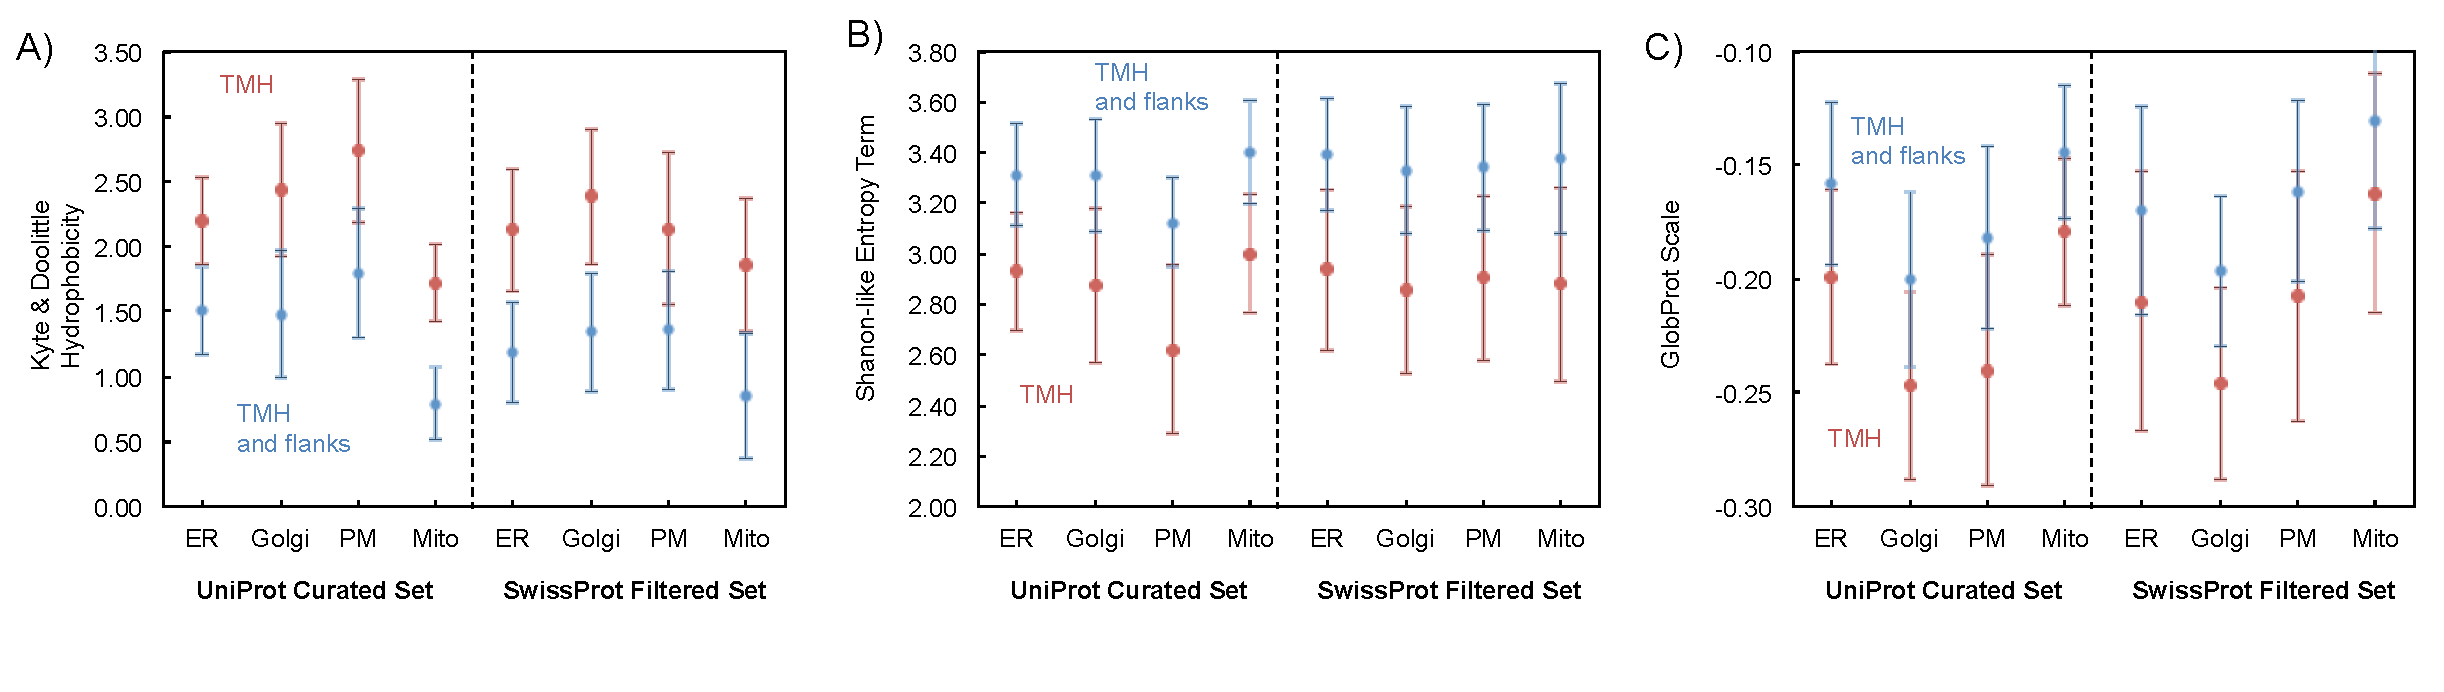
\includegraphics[width=1\textwidth]{TA_chapter/organelle-averages}
\captionof{figure}[Average sequence-based biochemical values of organelle datasets from UniProt manually curated set and SwissProt automatically filtered dataset.]
{\textbf{Average sequence-based biochemical values of organelle datasets from UniProt manually curated set and SwissProt automatically filtered dataset.}

A) The average hydrophoicity values from the Kyte \& Doolittle scale~\cite{Kyte1982}, B) the average sequence entropy~\cite{Shannon1948} (see methods) and C) the GlobProt scale~\cite{Linding2003} for both the \gls{tmh} and the \gls{tmh}$\pm$5 residues.
Values are shown for both the UniProt manually curated set and the SwissProt filtered set.
In the UniProt manually curated set we compare \gls{ta} proteins from the~\gls{er} (N=400) to the Golgi (N=82), the~\gls{pm} (N=37), and the mitochondria (N=401).
For the SwissProt filtered set we compare \gls{ta} proteins from the~\gls{er} (N=98) to the Golgi (N=82), the~\gls{pm} (N=157), and the mitochondria (N=65).
Error bars are shown at $\pm 1 \sigma$ from the mean of the respective dataset.
}

\label{fig:average_organelle_factors_ta}
\end{figure}

%\subsection{SNAREs are consistently more hydrophobic across the entire \gls{tmh}}
% Average lines for figure, table for stats

%~\gls{snare} proteins were noted to have more of the most hydrophobic amino acids than the general population of tail anchors~\cite{Kalbfleisch2007}.
%We exploit the difference by mapping the hydrophobicity of the transmembrane domains from a novel list of potential~\gls{ta} proteins generated in this study onto the experimentally validated~\gls{ta} hydrophobicity plot compiled by Kalbfleisch et al. published in Traffic 2007 (8: 1687-1694).
%This method has revealed potential~\gls{ta}~\gls{snare}s with~\gls{snare} motif domains that may not appear in conventional screening.

\subsection{Spontaneous insertion may be achieved by polar patches in the \gls{tmh}}
%Spont TA lines against background dataset.

%In addition, predicted insertion machinery dependent TAs with TMHs that are more polar on average than spontaneously inserting~\gls{ta} protein cytochrome b5 have been highlighted.

%move on to case studies involving spontaneous insertion?


%Our experimental collaborators in Stephen High’s group are interested in a small group of tail-anchored proteins that have very polar trans-membrane domains and are capable of liposome membrane insertion without insertion machinery, also known as spontaneous insertion.
%They have found that chimeric synaptobrevin, one of the first identified \gls{snare} proteins, is capable of spontaneous insertion if the tail anchor domain is replaced by the \gls{tm} domains belonging to a protein of known spontaneously inserting domains.
%Their studies have moved the focus of spontaneous insertion away from the loop regions and onto the physicochemical factors of the \gls{tmh} itself.


\section{Discussion}

Given the large biochemical distinction between \gls{ta} proteins with different terminal destinations, it is tempting to conclude that \gls{tmh}s contain the necessary biological factors to determine their targetting.
It is indeed possible that our observations are adaptations to the membrane environment, and this would not be unreasonable, except that \gls{ta} proteins would be expected to experience similar adaptations at a species level, for which at this sample size such an effect is unobservable.
Here, we postulate that there is indeed biological information held within the \gls{tmh} itself that allows the protein to be specifically targetted to a destiantion.
This is almost certainly aided by other factors and is part of a system with several redundant mechanisms.

Signal anchored proteins, proteins that contain a single hydrophobic segment that serves as both a mitochondrial targeting signal and a membrane anchor, as well as tail-anchored proteins have been shown to be able to spontaneously insert into the membrane independently from the translocon~\cite{Elisa2012, Lan2000, Colombo2009}.
The idea that \gls{snare} proteins are modular and capable of spontaneous insertion has significant implications for both biomedical application in liposome-based drug delivery and can aid future research for testing complex biological molecular networks~\cite{Allen2013, Nordlund2014}.

\section{Methods}

\subsection{Building a List of Tail-Anchors}
Steps carried out by Kalbfleisch \textit{et al.} published in Traffic 2007 (8: 1687\-1694)~\cite{Kalbfleisch2007}, were recreated using up to date tools.
Whilst their study focussed on the human proteome, here we take into account the entire TrEMBL and Swiss-Prot database and then stratify the datasets by the organism at the end of the pipeline.

\subsubsection{Swiss-Prot Tail Anchored Dataset According to Filters}
There were 557012 protein records downloaded from Swiss-Prot via UniProt~\cite{TheUniProtConsortium2014} (Downloaded 24--04--2018).
106149~\gls{tmh}s (\url{TRANSMEM} annotation) were found between 76953 records (\url{annotation:(type:transmem) AND reviewed:no}).
This keyword is contained in a record according to either experimental evidence~\cite{TheUniProtConsortium2014} or a robust meta-analysis of~\gls{tmh} prediction using TMHMM~\cite{Krogh2001}, Memsat~\cite{Jones2007}, Phobius~\cite{Kall2004,Kall2007} and the hydrophobic moment plot method of Eisenberg and co-workers~\cite{Eisenberg1984}.
11141 of those records had only a single~\gls{tmh}.
11110 of those~gls{tmh}s were within the length thresholds of 16 to 30 residues (None of those had the annotation for splice isoforms according to \url{NON_TER} annotation).
5548 of those had had no~\gls{sp} annotation (\url{SIGNAL}).
4332 of those had annotation (based on \url{TOPO_DOM} annotation) that the N terminal was cytoplasmic.
615 of those had the~\gls{tmh} within 25 residues of the C terminal, the same threshold used by Kalbfleisch and their coworkers~\cite{Kalbfleisch2007}.
Running CD-Hit 4.5.3 on the WebMGA webserver~\cite{Huang2010, Wu2011} at 90\% identical sequence at 90\% coverage thresholds resulted in 443 representative proteins.
This threshold was chosen as a compromise between avoiding over-representation of a certain protein and maintaining a viable sample size.

From this representative list, 46 were Archaeal, 66 were bacterial, and 320 were Eukaryotic and 11 came from dsDNA viruses.
When counting proteomes with greater than 20 records, 49 belonged to the \textit{A. thaliana} proteome, 48 to Mouse, 46 to the human proteome, 24 to \textit{S.cerevisiae}. %19 from RAT!

65 were annotated under the Mitochondrion location (query \url{locations:(location:"Mitochondrion [SL-0173]")}), 157 in the \gls{pm} (query \url{locations:(location:"Cell membrane [SL-0039]")}, 82 in the Golgi (query \url{locations:(location:"Golgi apparatus [SL-0132]")}), and 98 in the \gls{er} (query \url{locations:(location:"Endoplasmic reticulum [SL-0095]"}).

\subsubsection{TrEMBL Tail Anchored Dataset According to Filters}
111425234 records were storeed in the TrEMBL database at time of download (Downloaded 25--04--2018).
22107826 of those contained \url{TRANSMEM} annotation (\url{annotation:(type:transmem) AND reviewed:no}).
18053 of these were single-pass proteins.
All of these were within the length restrictions.
17973 of those did not contain a signal sequence when looking for \url{SIGNAL} annotation.
5157 of those contained a cytoplasmically located N terminal according to \url{TOPO_DOM} annotation.
155 records had a~\gls{tmh} within 15 residues of the C terminal residue.
In those record's annotations, no more than 1 appeared in any given species, so they were omited from the Swiss-Prot list sequence redundancy protocol to avoid representing a well annotated record with a poorly annotated record.

\subsubsection{UniProt Curated List}
A query for \url{locations:(location:"Single-pass type IV membrane protein [SL-9908]")} was used in UniProt which returned 2460 UniProtKB IDs; 463 Swiss-Prot results and 1997 TrEMBL results.
Running these records through CD-HIT at 90\% redundancy yielded 309 Swiss-Prot records and 808 TrEMBL records~\cite{Huang2010, Wu2011}.
Of those, 987 proteins from 973 records (308 from Swiss-Prot, and 665 from TrEMBL) had the \url{TRANSMEM} annotation indicating a bone fide~\gls{tmh}.
No further filters were applied to this list.
Proteomes represented by more than 20 records include \textit{A. thaliana} (60 records), Humans (38), Mouse (37), and \textit{S. cereveisiae} (31). % and 20 to Rat.

401 were annotated under the Mitochondrion location (query \url{locations:(location:"Mitochondrion [SL-0173]")}) 39 from Swissprot and 362 automatically assigned in TrEMBL.
401 in the \gls{er} (query \url{locations:(location:"Endoplasmic reticulum [SL-0095]"}), 98 from SwissProt and 303 automatically annotated in TrEMBL.
1 TrEMBL record (A0A1E5RT24) in the \gls{er} set contained an ``X'' residue in the C terminal flank and was omitted from the analyses.
Two subcellular location datasets had no automatically ascribed records and only contained manually annoted SwissProt records; 37 in the \gls{pm} (query \url{locations:(location:"Cell membrane [SL-0039]")}, and 82 in the Golgi (query \url{locations:(location:"Golgi apparatus [SL-0132]")}).

\subsubsection{Remapping Previous Dataset}
189 of the 411 proteins from the previous study~\cite{Kalbfleisch2007} were successfully mapped to 222 UniProtKB IDs using the UniProt mapping tools with the RefSeq Protein to UniProtKB option~\cite{TheUniProtConsortium2014}.

\subsection{Calculating Hydrophobicity}
Windowed hydrophobicity was calculated using a window length of 5 residues, and half windows were permitted.
Average hydrophobicity takes the total of the raw amino acid hydrophobicity values and divides them by the number of amino acids in the slice.
Values reported in the results are based on the Kyte \& Doolittle scale~\cite{Kyte1982} which is based on the water\---vapour transfer free energy and the interior-exterior distribution of individual amino acids.
%Hydrophobicity values were also validated by the White and Wimley scale~\cite{White1999}, the Hessa scale~\cite{Hessa2005}, and the Eisenberg scale~\cite{Eisenberg1984}.

\subsection{Calculating Sequence Entropy}
Sequence entropy, is essentially an estimate of the linguistic entropy of a string.
In the context of biology, it can be thought of as an estimation of the non-randomness of a sequence.
Sequence complexity can be used to analyse DNA sequences~\cite{Pinho2013, Oliver1993, Troyanskaya2002}, and is a component of the TMSOC z-score which can predict function beyond anchorage of a \gls{tmh}~\cite{Wong2011, Wong2012, Baker2017}.
here we focus on the analysis of the complexity of a sequence in protein sequences.

Broadly speaking, the information theory entropy of a linguistic string can be defined as in equation~\ref{simpleentropy2}, and we treat the protein sequence \gls{tmh} as a string with or without its flanking regions.

\begin{equation} \label{simpleentropy2}
	H(S)=-{\sum_{i=1}^n {p_i\log_s(p_i)}}
\end{equation}

Where H is the entropy of a sequence (S), and $p_i$ is the probability of a character $i$ through each position (n) in S. This allows us to quantify the average relative information density held within a string of information~\cite{Shannon1948}.

\subsection{Statistics}

The null hypothesis of homogeneity of two distributions was examined with the~\gls{ks}, the~\gls{kw} and the 2-sampled T-test statistical tests.
These tests were all ran through the Python scipy stat package v0.17 python package~\cite{VanderWalt2011}.
To note, the~\gls{ks} test scrutinises for significant maximal absolute differences between distribution curves; the~\gls{kw} test is after skews between distributions and the student t-test statistical test checks the average difference between distributions.

Since the ``P‑value'' is a product of a fraction of a permutated set that exponentially increases as N increases, the P-value is a strong function of N.
We rely on the (absolute) Bahadur slope ($B$) as a measure of distance between two distributions~\cite{Bahadur1967, Bahadur1971, Sunyaev1998, Baker2017}:

\begin{equation} \label{eq:bahadur2}
B=\frac{|\ln(P~value)|}{N}
\end{equation}

The larger the absolute Bahadur slope, the greater the difference between the two distributions.
